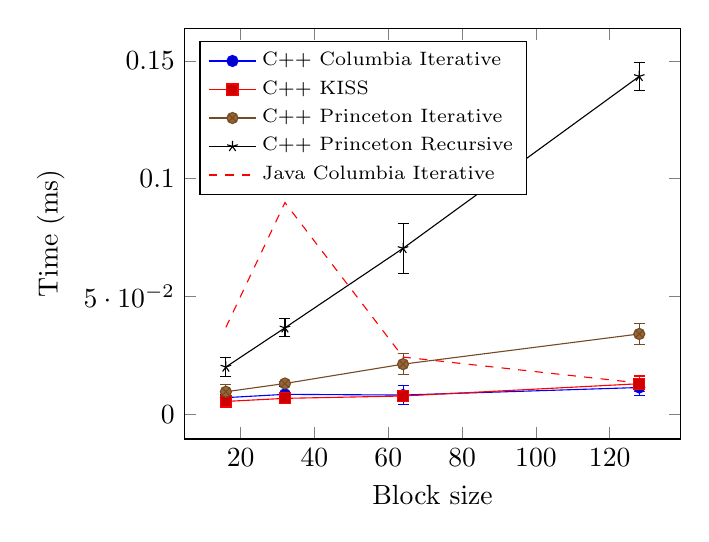
\begin{tikzpicture}
\begin{axis}[xlabel={Block size},ylabel={Time (ms)},width=0.65\linewidth,legend pos=north west,scaled y ticks = false,legend cell align=left,legend style={font=\scriptsize}]
\addplot+[error bars/.cd, y dir=both,y explicit] coordinates {
(16, 0.0072) +- (0.0012, 0.0012)
(32, 0.0086) +- (0.0034, 0.0034)
(64, 0.0083) +- (0.0041, 0.0041)
(128, 0.0115) +- (0.0033, 0.0033)
};
\addplot+[error bars/.cd, y dir=both,y explicit] coordinates {
(16, 0.0056) +- (0.0013, 0.0013)
(32, 0.0069) +- (0.0005, 0.0005)
(64, 0.0079) +- (0.0009, 0.0009)
(128, 0.0131) +- (0.0033, 0.0033)
};
\addplot+[error bars/.cd, y dir=both,y explicit] coordinates {
(16, 0.0097) +- (0.0032, 0.0032)
(32, 0.0132) +- (0.0009, 0.0009)
(64, 0.0214) +- (0.0044, 0.0044)
(128, 0.0342) +- (0.0045, 0.0045)
};
\addplot+[error bars/.cd, y dir=both,y explicit] coordinates {
(16, 0.0202) +- (0.0039, 0.0039)
(32, 0.0368) +- (0.0038, 0.0038)
(64, 0.0705) +- (0.0105, 0.0105)
(128, 0.1434) +- (0.0059, 0.0059)
};
\addplot+[style=dashed,color=red,mark=none] coordinates {
(16, 0.0370) +- (0.0055, 0.0055)
(32, 0.0899) +- (0.0169, 0.0169)
(64, 0.0244) +- (0.0637, 0.0637)
(128, 0.0134) +- (0.0005, 0.0005)
};
\legend{C++ Columbia Iterative , C++ KISS , C++ Princeton Iterative , C++ Princeton Recursive, Java Columbia Iterative}
\end{axis}
\end{tikzpicture}
